\usection{Lecture 15: Dynamic games with Incomplete information (cont.)}
\newsection
\subsection*{Logistics}
\begin{enumerate}
    \item Exam graded
    \item Project - 8 minute presentation and 2 minute Q and A
\end{enumerate}
\subsection*{Recap}
\begin{enumerate}
    \item Dynamic games with incomplete information
    \item Perfect Bayesian Equilibira - Beliefs and action profiles
    \item Signalling games
    \item Pooling equilibira and separated equilibria in signalling games
\end{enumerate}
\begin{aexample}{Costly signalling}{}
    The sender is a seller. The type indicates the quality of the product. \[
    t_1 = \rm{`good'}, t_2 = \rm{`bad'}.
    \]
    Based on this signal, the sender can send a message to the receiver (buyer). \[
        m_1 = \textrm{`warranty'}, m_2 = \textrm{`no warranty'}.
    \]
    
    \begin{center}
        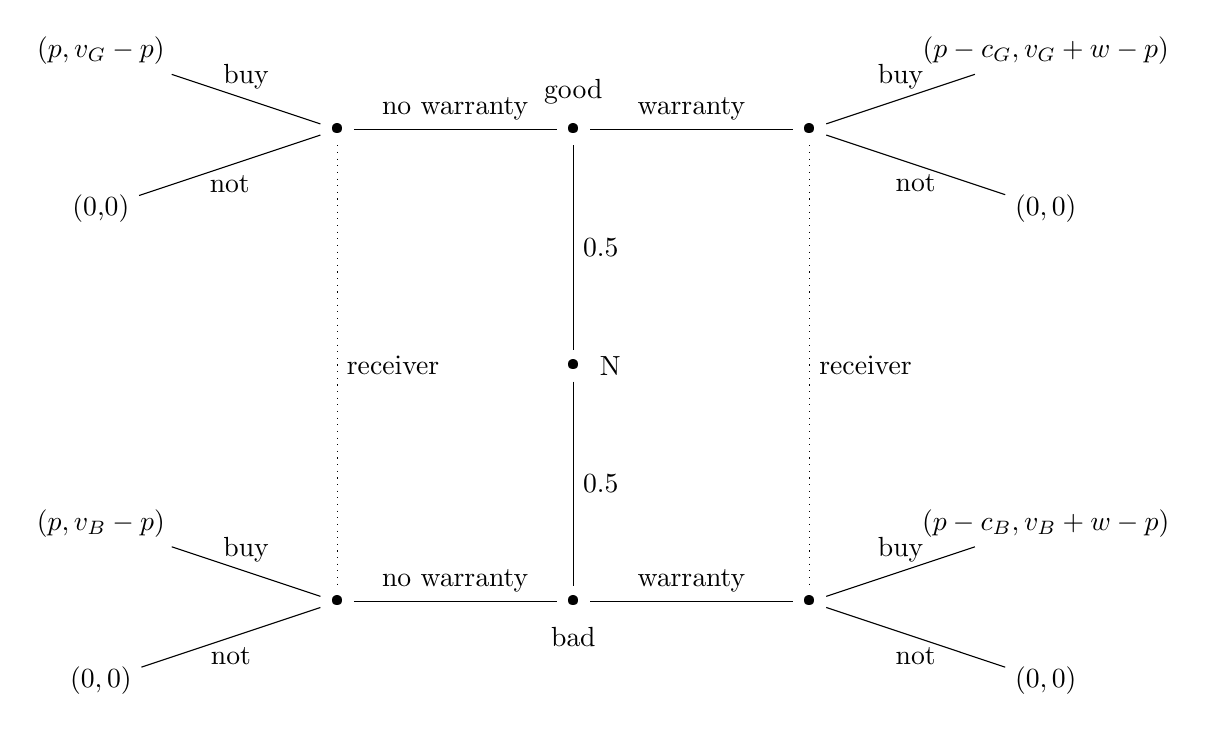
\begin{tikzpicture}
            \node[label={right:N}] (start) at (0,0){\textbullet};
            \node[label={above:good}] (good) at (0,3){\textbullet};
            \node[label={below:bad}] (bad) at (0,-3){\textbullet};
            \path (start) edgenode[midway,right]{0.5}(good);
            \path(start) edge node[midway,right]{0.5}(bad);

            \node (inv1) at (-3,3) {\textbullet};
            \node (inv2) at (-3,-3) {\textbullet};
            \node (inv3) at (3,3) {\textbullet};
            \node (inv4) at (3,-3) {\textbullet};

            \path[dotted] (inv1)edge node[midway, right]{receiver} (inv2);
            \path[dotted] (inv3)edge node[midway, right]{receiver} (inv4);
            

            \path (inv1) edge node[midway,above]{no warranty} (good);
            \path (inv2) edgenode[midway,above]{no warranty} (bad);
            \path (inv3) edge node[midway,above]{warranty}(good);
            \path (inv4) edge node[midway,above]{warranty}(bad);
            \node (one) at(-6,4){$(p,v_G-p)$};
            \node (two) at(-6,2){(0,0)};
            \node (three) at(-6,-2){$(p,v_B-p)$};
            \node (four) at(-6,-4){$(0,0)$};
            \node (five) at(6,4){$(p-c_G,v_G+w-p)$};
            \node (six) at(6,2){($0,0)$};
            \node (seven) at(6,-2){$(p-c_B,v_B+w-p)$};
            \node (eight) at(6,-4){$(0,0)$};
            \path (inv1) edge   node [midway, above] {buy} (one);
            \path (inv1) edge   node [midway, below ] {not } (two);
            \path (inv2) edge   node [midway, above] {buy} (three);
            \path (inv2) edge   node [midway, below ] {not } (four);
            \path (inv3) edge   node [midway, above] {buy} (five);
            \path (inv3) edge   node [midway, below ] {not } (six);
            \path (inv4) edge   node [midway, above] {buy} (seven);
            \path (inv4) edge   node [midway, below ] {not } (eight);

        \end{tikzpicture}
    \end{center}
    We are interested in the separating equilibira.
\end{aexample}

Suppose that the seller is providing warranty if and only if the type is good. We set $v_G+w-p>0$ and $v_B-p<0$,
so the buyer will buy if and only if warranty is provided. The seller will also not deviate from the strategy if $p-c_G>0$ and $p-c_B<0$. This means that we would need the price for a bad warranty is more costly.




\begin{aexample}{Cheap talk}{}
    The sender is a recommender. The type indicates the quality of the product. \[
    t_1 = \rm{`good'}, t_2 = \rm{`bad'}.
    \]
    Based on this signal, the sender can send a message to the receiver (buyer). \[
        m_1 = \textrm{`recommend'}, m_2 = \textrm{`do not recommend'}.
    \]
    The recommender gets a price of advertising $p$.
    \begin{center}
        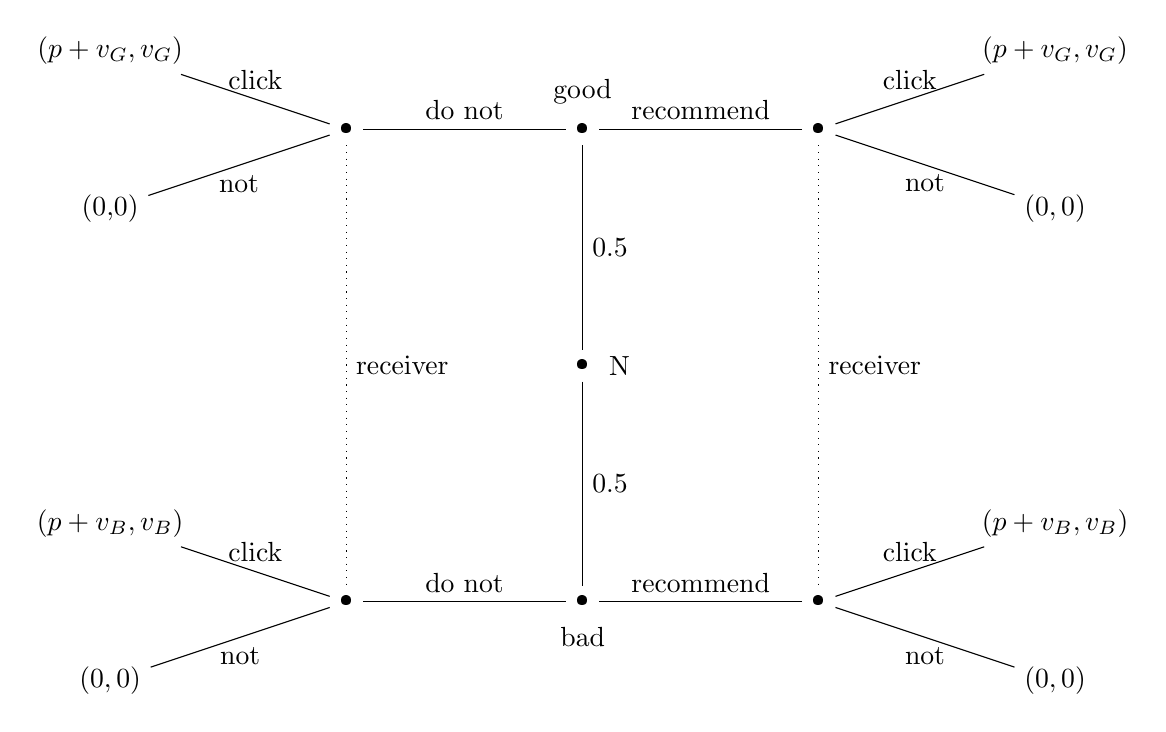
\begin{tikzpicture}
            \node[label={right:N}] (start) at (0,0){\textbullet};
            \node[label={above:good}] (good) at (0,3){\textbullet};
            \node[label={below:bad}] (bad) at (0,-3){\textbullet};
            \path (start) edgenode[midway,right]{0.5}(good);
            \path(start) edge node[midway,right]{0.5}(bad);

            \node (inv1) at (-3,3) {\textbullet};
            \node (inv2) at (-3,-3) {\textbullet};
            \node (inv3) at (3,3) {\textbullet};
            \node (inv4) at (3,-3) {\textbullet};

            \path[dotted] (inv1)edge node[midway, right]{receiver} (inv2);
            \path[dotted] (inv3)edge node[midway, right]{receiver} (inv4);
            

            \path (inv1) edge node[midway,above]{do not} (good);
            \path (inv2) edgenode[midway,above]{do not} (bad);
            \path (inv3) edge node[midway,above]{recommend}(good);
            \path (inv4) edge node[midway,above]{recommend}(bad);
            \node (one) at(-6,4){$(p+v_G,v_G)$};
            \node (two) at(-6,2){(0,0)};
            \node (three) at(-6,-2){$(p+v_B,v_B)$};
            \node (four) at(-6,-4){$(0,0)$};
            \node (five) at(6,4){$(p+v_G,v_G)$};
            \node (six) at(6,2){($0,0)$};
            \node (seven) at(6,-2){$(p+v_B,v_B)$};
            \node (eight) at(6,-4){$(0,0)$};
            \path (inv1) edge   node [midway, above] {click} (one);
            \path (inv1) edge   node [midway, below ] {not } (two);
            \path (inv2) edge   node [midway, above] {click} (three);
            \path (inv2) edge   node [midway, below ] {not } (four);
            \path (inv3) edge   node [midway, above] {click} (five);
            \path (inv3) edge   node [midway, below ] {not } (six);
            \path (inv4) edge   node [midway, above] {click} (seven);
            \path (inv4) edge   node [midway, below ] {not } (eight);

        \end{tikzpicture}
    \end{center}

    Notice now that there is no cost of signalling. Is it still possible to create a separating equilibrium?
\end{aexample}
We want (not recommend, not click) for bad and (recommend, click) for good. Thus, we need $v_G>0$ and $v_B<0$. For the recommender to not deviate, we also need $p+v_G>0$ and $p+v_B<0$

\begin{aexample}{Bayesian Persuasion}{}
    \begin{center}
        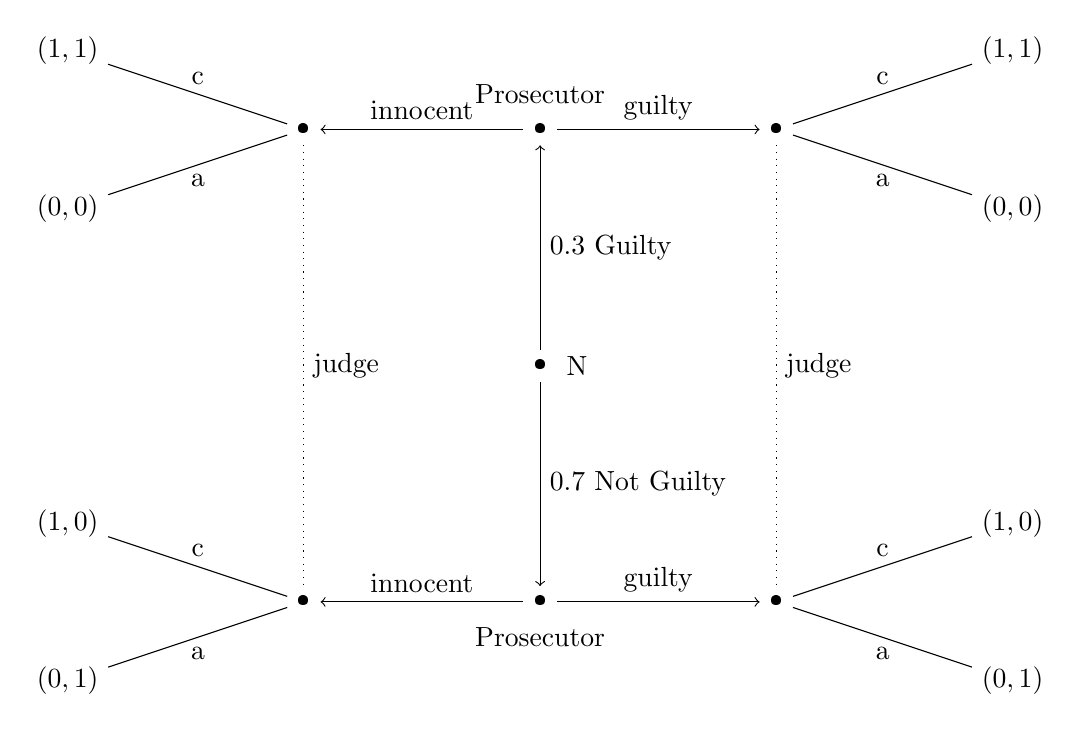
\begin{tikzpicture}
            \node[label={right:N}] (start) at (0,0){\textbullet};
            \node[label={above:Prosecutor}] (good) at (0,3){\textbullet};
            \node[label={below:Prosecutor}] (bad) at (0,-3){\textbullet};
            \path[->] (start) edgenode[midway,right]{0.3 Guilty}(good);
            \path[->](start) edge node[midway,right]{0.7 Not Guilty}(bad);

            \node (inv1) at (-3,3) {\textbullet};
            \node (inv2) at (-3,-3) {\textbullet};
            \node (inv3) at (3,3) {\textbullet};
            \node (inv4) at (3,-3) {\textbullet};

            \path[dotted] (inv1)edge node[midway, right]{judge} (inv2);
            \path[dotted] (inv3)edge node[midway, right]{judge} (inv4);
            

            \path[<-] (inv1) edge node[midway,above]{innocent} (good);
            \path[<-] (inv2) edgenode[midway,above]{innocent} (bad);
            \path[<-] (inv3) edge node[midway,above]{guilty}(good);
            \path[<-] (inv4) edge node[midway,above]{guilty}(bad);
            \node (one) at(-6,4){$(1,1)$};
            \node (two) at(-6,2){$(0,0)$};
            \node (three) at(-6,-2){$(1,0)$};
            \node (four) at(-6,-4){$(0,1)$};
            \node (five) at(6,4){$(1,1)$};
            \node (six) at(6,2){($0,0)$};
            \node (seven) at(6,-2){$(1,0)$};
            \node (eight) at(6,-4){$(0,1)$};
            \path (inv1) edge   node [midway, above] {c} (one);
            \path (inv1) edge   node [midway, below ] {a } (two);
            \path (inv2) edge   node [midway, above] {c} (three);
            \path (inv2) edge   node [midway, below ] {a } (four);
            \path (inv3) edge   node [midway, above] {c} (five);
            \path (inv3) edge   node [midway, below ] {a } (six);
            \path (inv4) edge   node [midway, above] {c} (seven);
            \path (inv4) edge   node [midway, below ] {a } (eight);

        \end{tikzpicture}
    \end{center}
\end{aexample}
There is no stable separating equilibirum. If the judge charges for only guilty people, the prosecutor would pick guilty every time. Under this equilibirum, the judge acquits everyone so the payoff is $(0,0.7)$.
We want to find out what changes if the sender can `commit' to signalling strategy before Nature moves. I.e. the sender picks all guilty, or the sender picks separating guilty and innocent. The judge knows the prosecutor's strategy beforehand and can adapt. We see that it is better for the prosecutor to use a separating strategy.

The prosecutor can also use a mixed strategy to maximize profit. For guilty, signal `guilty' with probability 1. For innocent, signal `guilty' to `innocent' with odds $3:4$. Under this case, the probability that a person is guilty given a guilty signal is $0.5$. The judge acquits if and only if there is an innocent signal. This means we would convict $0.6$ of all people even if only $0.3$ of them are guilty.

\begin{remark}
    This equilibirum is only possible because the sender has to commit to a strategy beforehand.
\end{remark}

\subsection*{Bayesian Observation Learning}
Suppose there is an item that is available for buy. It is either good or bad for all agents with probability $1/2$ each. Each agent does not know the state of world (do not know if item is good or bad), but they get an IID signal (Bernoulli trials with accuracy $p>1/2$).
Each agent sequentially makes decisions based on their signal and the observations.
The payoff is $1$ for buying a good item, $-1$ for buying a bad item, and $0$ for not buying.
The first agent follows its signal. The remaining agents update according to Bayes' rule. Second agent uses `popular vote' between him and the first agent.